
\section{Nico Ekklesia Sembiring}
\subsection{Buatlah fungsi untuk mendapatkan data langsung dari arduino}
\lstinputlisting[caption = Mendapatkan data dari Arduino., firstline=8, lastline=14]{src/5/Praktek/1174096/1174096_realtime.py}

\subsection{Buatlah fungsi untuk mendapatkan data langsung dari arduino dengan looping}
\lstinputlisting[caption = Mendapatkan data langsung dari Arduino dengan looping., firstline=8, lastline=15]{src/5/Praktek/1174096/1174096_save.py}

\subsection{Buatlah fungsi untuk mendapatkan data dari arduino dan langsung ditulis kedalam file csv}
\lstinputlisting[caption = Mendapatkan data dari Arduino dan langsung ditulis kedalam file CSV., firstline=16, lastline=30]{src/5/Praktek/1174096/1174096_realtime.py}

\begin{figure}[H]
	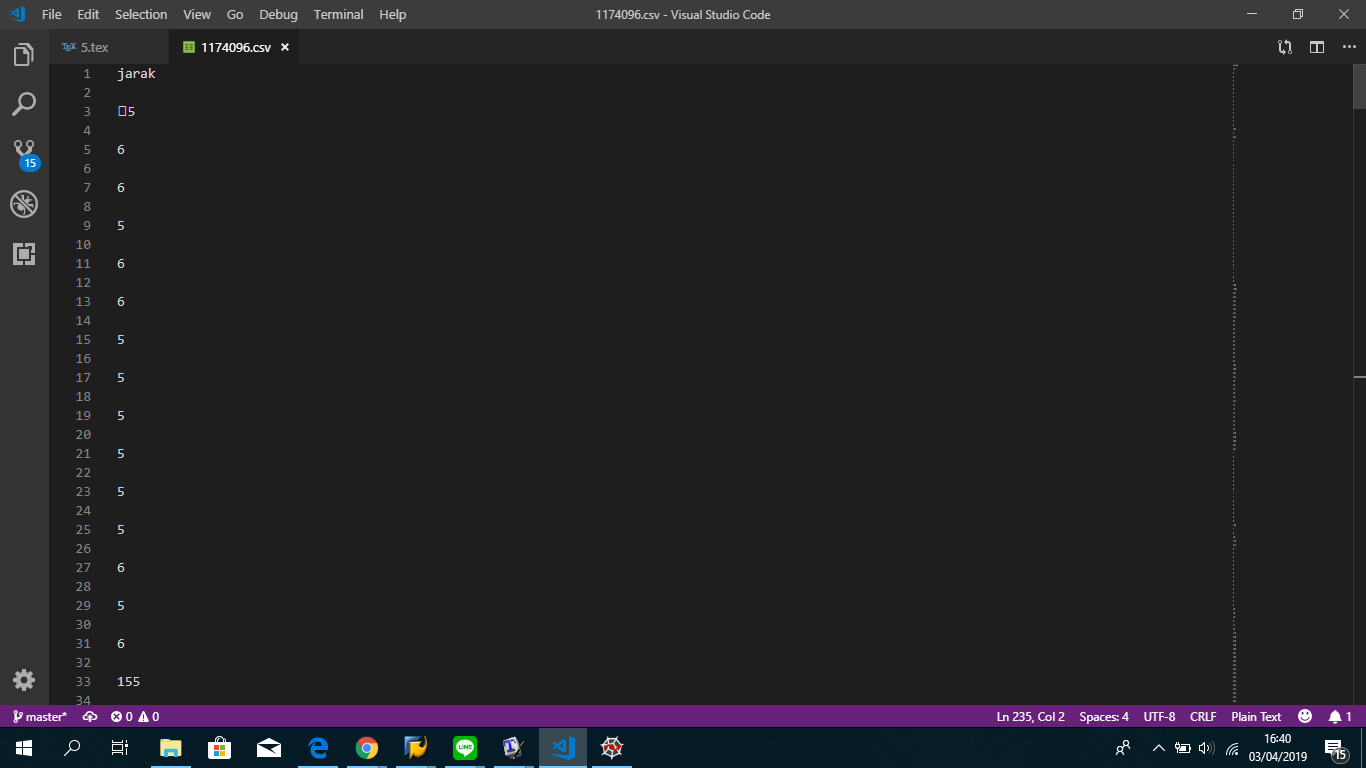
\includegraphics[width=9cm]{figures/5/Praktek/1174096/hasilcsv.png}
	\caption{Hasil dari pembacaan data dari arduino dalam bentuk file CSV.}
	\centering
\end{figure}

\subsection{Buatlah fungsi untuk membaca file csv hasil arduino dan mengembalikan ke fungsi}
\lstinputlisting[caption = Membaca file CSV hasil Arduino dan mengembalikan fungsi., firstline=8, lastline=16]{src/5/Praktek/1174096/1174096_csv.py}

\subsection{Pengecekan Plagiarisme Praktek}
\begin{figure}[H]
	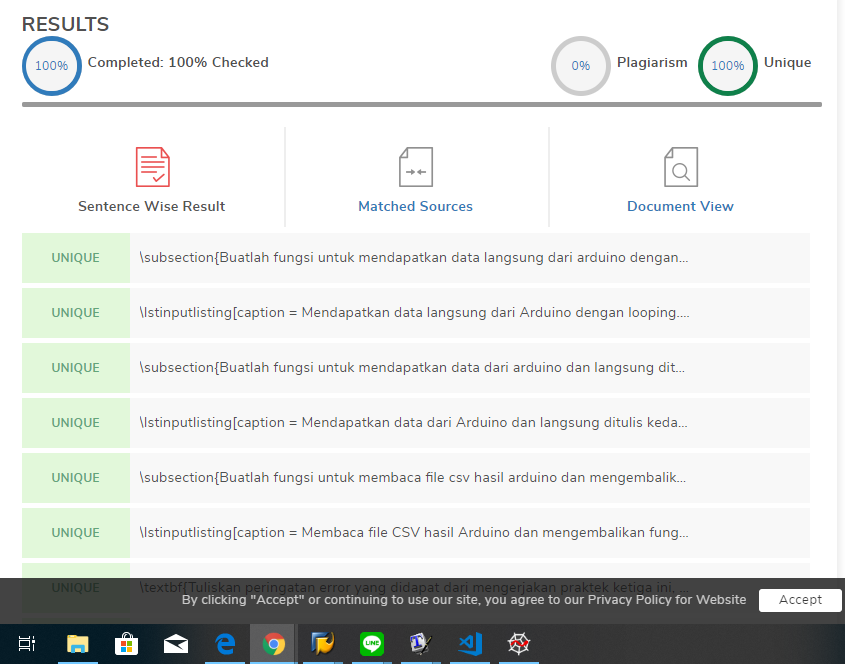
\includegraphics[width=9cm]{figures/5/Praktek/1174096/Plagiarismepraktek.png}
	\centering
\end{figure}

\subsection{Ketrampilan Penanganan Error}
\textbf{Tuliskan peringatan error yang didapat dari mengerjakan praktek ketiga ini, dan jelaskan cara penanganan error tersebut. dan Buatlah satu fungsi yang menggunakan gunakan try except untuk menanggulangi error tersebut}

Peringatan error yang saya temui pada praktek Chapter 5 ini, adalah:
\begin{itemize}
	\item Name Error
	NameError adalah exception yang terjadi ketika kode melakukan eksekusi terhadap local name atau global name yang tidak terdefinisi oleh perangkat. Solusi yang dapat dilakukan adalah dengan memastikan variabel atau fungsi yang dipanggil ada atau tidak salah ketik.
	
	\item Syntax Errors
	Syntax Errors adalah suatu keadaan saat  terjadi kesalahan penulisan pada kode python. Cara memperbaikinya adalah dengan memperbaiki penulisan kode yang salah.
	
	\item Type Error
	TypeError adalah exception yang terjadi pada saat dilakukannya eksekusi terhadap suatu operasi atau fungsi dengan type object yang tidak sesuai. Cara yang dilakukan untuk mengatasinya error ini adalah mengkoversi varibelnya sesuai dengan tipe data yang akan digunakan.
\end{itemize}

\textbf{Penanggulangan Error menggunakan Try Except}
\lstinputlisting[caption = Penanggulangan error menggunakan Try Except., firstline=8, lastline=23]{src/5/Praktek/1174096/1174096.py}

\subsection{Pengecekan Plagiarisme Penanganan Error}
\begin{figure}[H]
	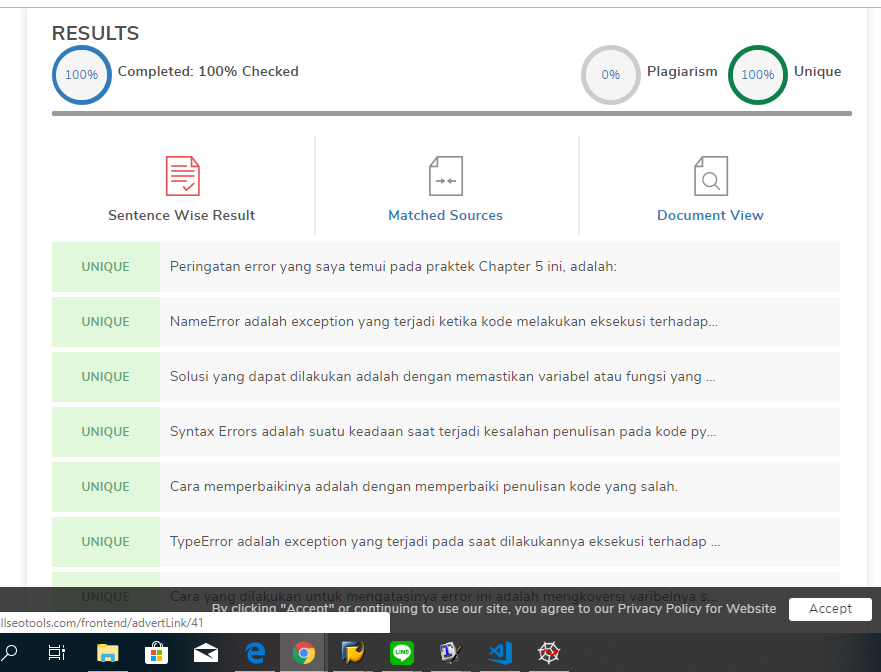
\includegraphics[width=9cm]{figures/5/Praktek/1174096/Plagiarismeerror.png}
	\centering
\end{figure}

\section{Habib Abdul Rasyid}
{\Large \textbf{Ketrampilan Pemrograman}}
\subsection{Soal No. 1}
Buatlah  fungsi  (file  terpisah/library  dengan  nama  NPMrealtime.py)  untuk mendapatkan data langsung dari arduino!
\lstinputlisting[caption = Fungsi untuk mendapatkan data dari Arduino., firstline=1, lastline=14]{src/5/Praktek/1174002/1174002realtime.py}


\subsection{Soal No. 2}
Buatlah fungsi (file terpisah/library dengan nama NPMsave.py) untuk mendapatkan data langsung dari arduino dengan looping!
\lstinputlisting[caption = Fungsi untuk mendapatkan data langsung dari Arduino dengan looping., firstline=1, lastline=8]{src/5/Praktek/1174002/1174002save.py}

\subsection{Soal No. 3}
Buatlah  fungsi  (file  terpisah/library  dengan  nama  NPMrealtime.py) untuk mendapatkan data dari arduino dan langsung ditulis kedalam file csv!
\lstinputlisting[caption = Fungsi untuk mendapatkan data dari Arduino dan langsung ditulis kedalam file CSV., firstline=16, lastline=30]{src/5/Praktek/1174002/1174002realtime.py}

\begin{figure}[H]
	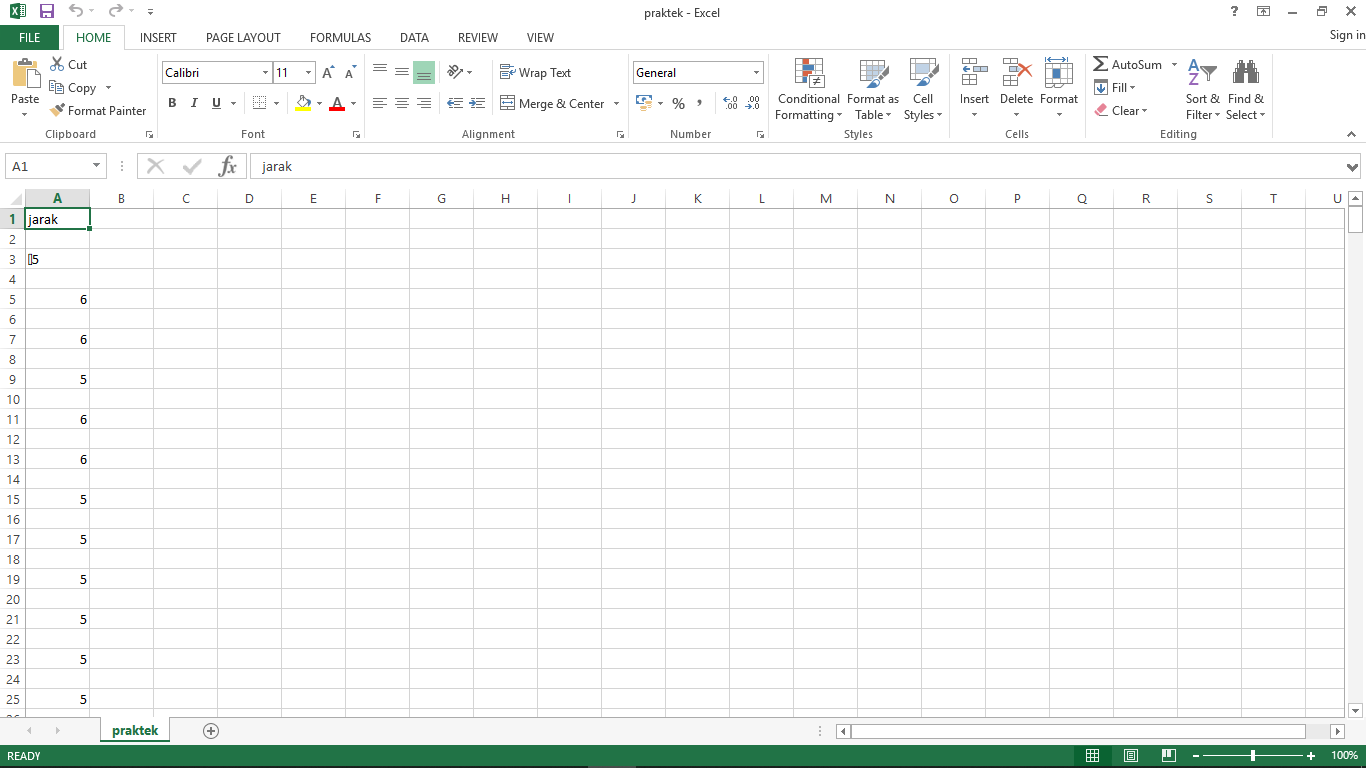
\includegraphics[scale=0.2]{figures/5/Praktek/1174002/csv.png}
	\centering
	\caption{Hasil dari pembacaan fungsi untuk mendapatkan data dari Arduino dan langsung ditulis kedalam file CSV.}
\end{figure}

\subsection{Soal No. 4}
Buatlah fungsi (file terpisah/library dengan nama NPMcsv.py) untuk membaca file csv hasil arduino dan mengembalikan ke fungsi!
\lstinputlisting[caption = Fungsi untuk membaca file CSV hasil Arduino dan mengembalikan fungsi., firstline=1, lastline=9]{src/5/Praktek/1174002/1174002csv.py}

\subsection{Cek Plagiat Praktek}
\begin{figure}[H]
	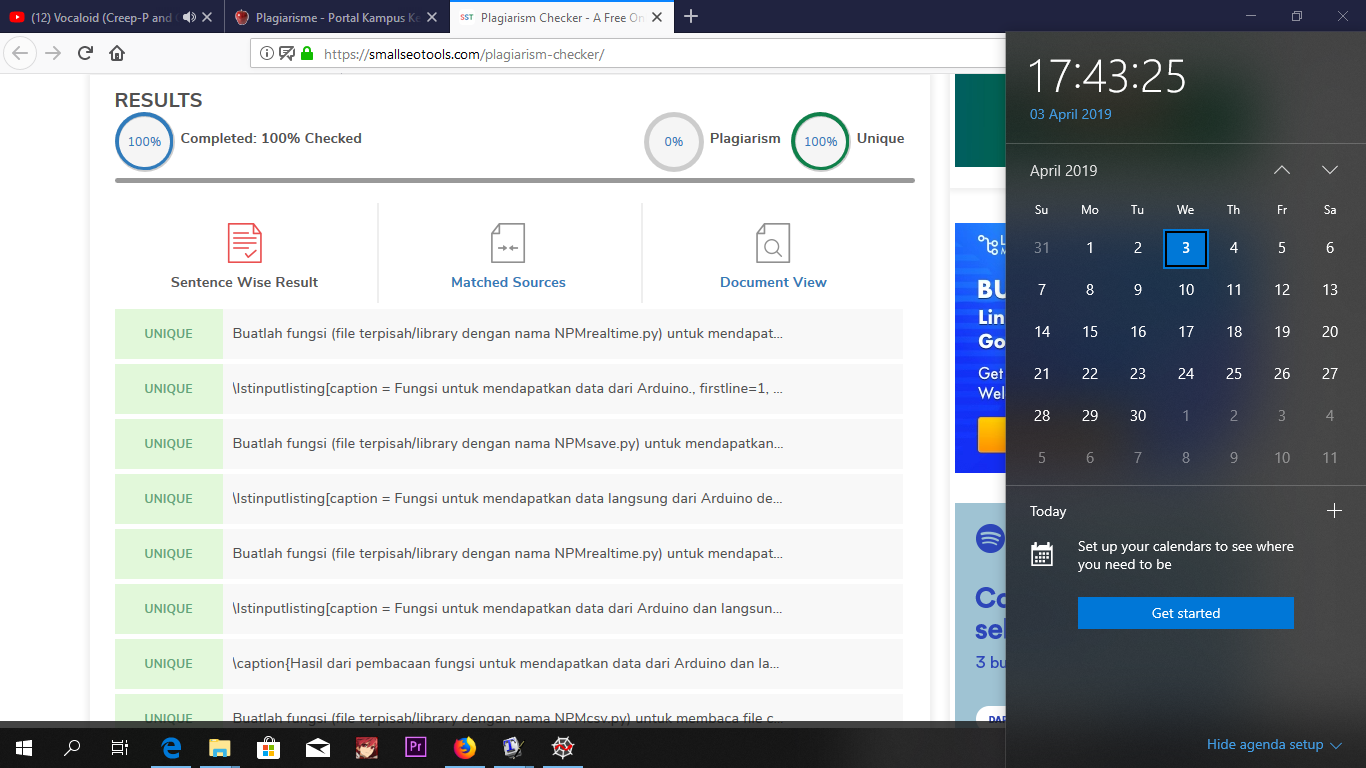
\includegraphics[scale=0.2]{figures/5/Praktek/1174002/plagiat.png}
	\caption{Plagiarisme Habib}
	\centering
\end{figure}

\hfill \break
{\Large \textbf{Ketrampilan Penanganan Error}}

\subsection{Soal No. 1}
Tuliskan  peringatan  error  yang  didapat  dari  mengerjakan  praktek  kelima  ini, dan  jelaskan  cara  penanganan  error  tersebut.   dan  Buatlah  satu  fungsi  yang menggunakan try except untuk menanggulangi error tersebut.

\hfill \break
Peringatan error di praktek kelima ini, yaitu:
\begin{itemize}
	\item Syntax Errors
	Syntax Errors adalah suatu keadaan saat kode python mengalami kesalahan penulisan. Solusinya adalah memperbaiki penulisan kode yang salah.
		
	\item Type Error
	TypeError adalah exception yang akan terjadi apabila pada saat dilakukannya eksekusi terhadap suatu operasi atau fungsi dengan type object yang tidak sesuai. Solusi dari error ini adalah mengkoversi varibelnya sesuai dengan tipe data yang akan digunakan.
\end{itemize}

\hfill \break
Fungsi yang menggunakan try except untuk menanggulangi error.

\lstinputlisting[caption = Fungsi untuk menanggulangi error menggunakan Try Except., firstline=1, lastline=16]{src/5/Praktek/1174002/1174002.py}


\section{Tomy Prawoto}
\subsection{Soal 1}
Isi jawaban soal ke-1

Kalau mau dibikin paragrap \textbf{cukup enter aja}, tidak usah pakai \verb|par| dsb

%\subsection{Soal 2}
%Isi jawaban soal ke-2

%\subsection{Soal 3}
%Isi jawaban soal ke-3
